\chapter*{Appendix}
\addcontentsline{toc}{chapter}{Appendix}

\section*{Complete Handcard data plots}
\label{hc_appendix}

\begin{figure}[h]
\begin{center}
    \makebox[\linewidth][c]{
    \begin{subfigure}[b]{.7\textwidth}
        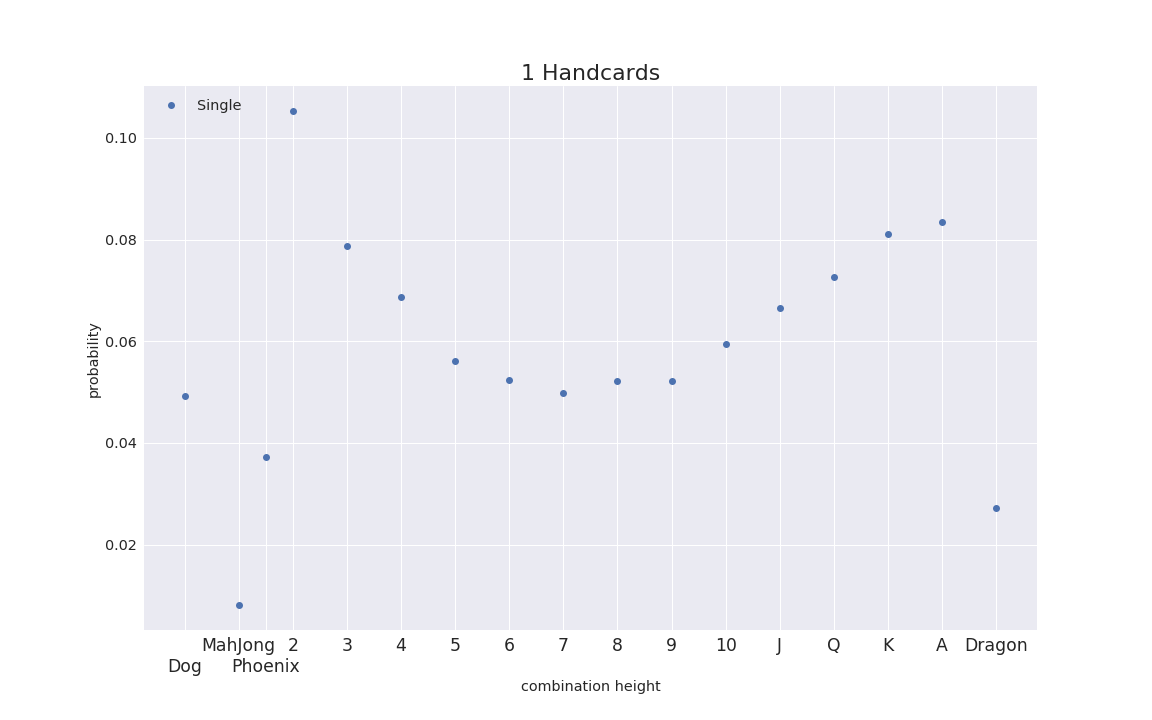
\includegraphics[width=\textwidth]{images/det/type_for_len_1}
        \caption{Handcards of length 1}
    \end{subfigure}
    \hspace{-60px}
    \begin{subfigure}[b]{.7\textwidth}
        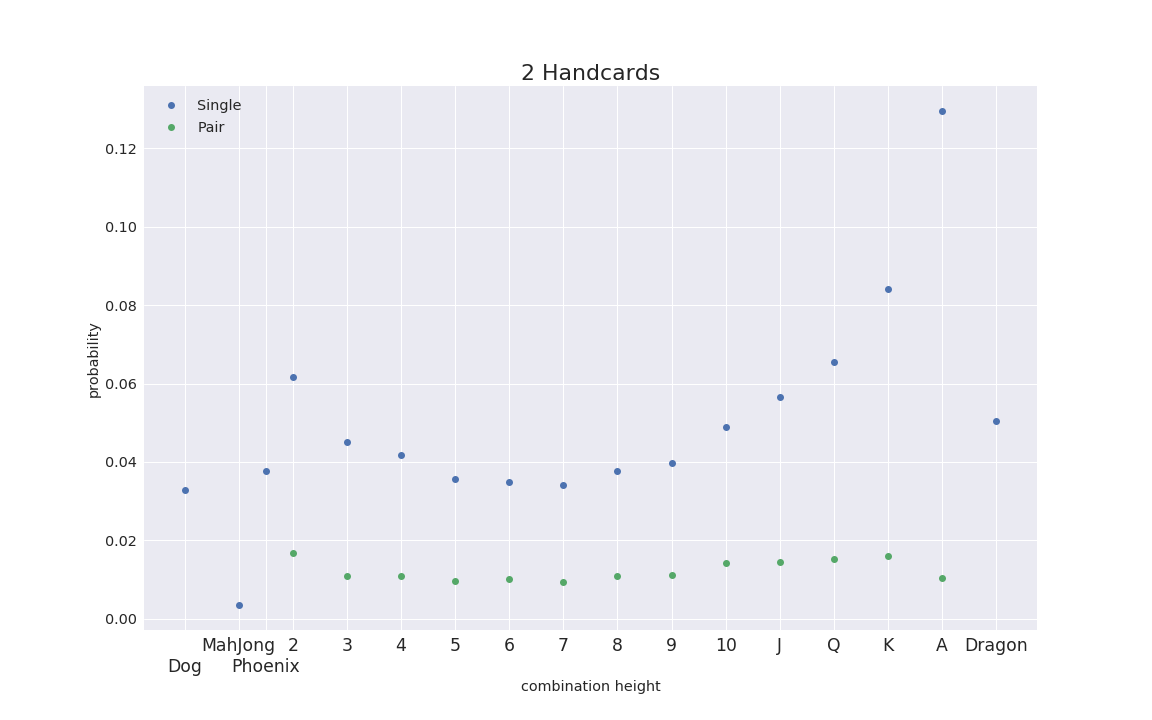
\includegraphics[width=\textwidth]{images/det/type_for_len_2}
        \caption{Handcards of length 2}
    \end{subfigure}
    }
\end{center}
\end{figure}

\foreach \x/\y in {3/4,5/6,7/8,9/10,11/12,13/14}{
    \begin{figure}[h]\ContinuedFloat
    \begin{center}
        \makebox[\linewidth][c]{
        \begin{subfigure}[b]{.7\textwidth}
            \includegraphics[width=\textwidth]{images/det/type_for_len_\x}
            \caption{Handcards of length \x}
        \end{subfigure}
        \hspace{-60px}
        \begin{subfigure}[b]{.7\textwidth}
            \includegraphics[width=\textwidth]{images/det/type_for_len_\y}
            \caption{Handcards of length \y}
        \end{subfigure}
        }\\
    \end{center}
    \end{figure}
}

\clearpage
